%% -*- coding: utf-8 -*-
\documentclass[12pt,pagesize,paper=192mm:108mm,landscape]{scrbook} 
%1920x1080 1280x720
\areaset[current]{192mm}{108mm}
\usepackage{calc}
\usepackage[T2A]{fontenc}
\usepackage[utf8]{inputenc}
\usepackage[english,russian]{babel}
\usepackage{microtype}
\usepackage{misccorr}
\usepackage{cmap}
%\usepackage[unicode=true]{hyperref}
\usepackage{graphicx}
\usepackage{amssymb}
\usepackage{amsmath}
%\usepackage{srcltx}
\usepackage{textcomp}
\usepackage{xspace}
%научные символы и смайлики \smiley \frownie
\usepackage{wasysym}
\usepackage{ccicons}
\begin{document}
\begin{titlepage}
  \vspace*{-0.5em}
  \begin{center}    
    % \hspace*{3em}
    % \begin{minipage}[t]{3em}
    %   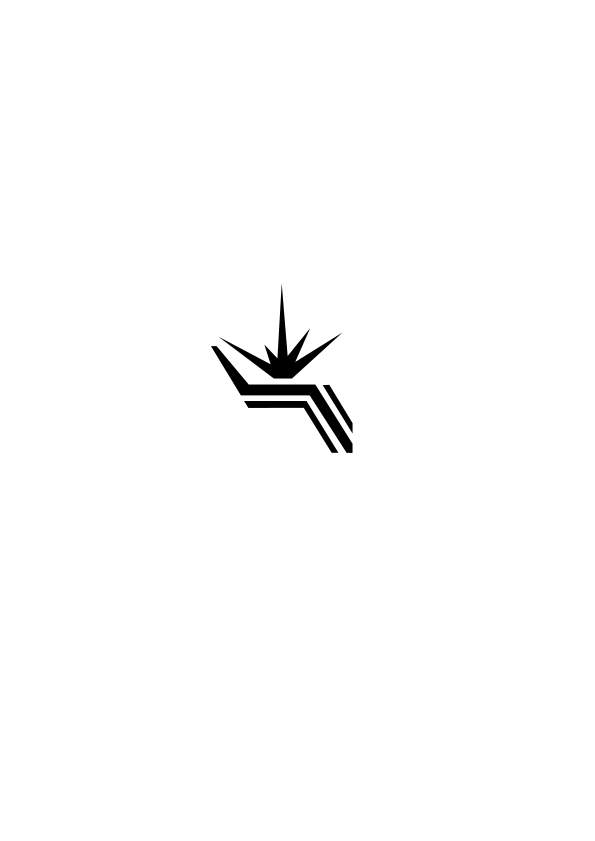
\includegraphics[width=\textwidth]{../BINP-logo}
    % \end{minipage}\hfill
    % \begin{minipage}{0.23\linewidth}
    % 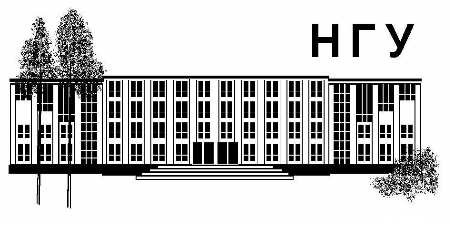
\includegraphics[width=\textwidth]{../NSU-logo}
    % \end{minipage}
    % \hfill
    % \hspace*{6em}

    % Кафедра теоретической физики физического факультета НГУ
    % \medskip

    % \Large
    % Профессор Грабовский А.\,В.
    % \smallskip

    % \huge
    % \textbf{Общая теория относительности}
    % \smallskip

    \vfill
    \Large
    Задание № 3
    \bigskip

    \normalsize
    \begin{minipage}{0.65\linewidth}
Показать следующие свойства тензора Римана:
\begin{enumerate}
\item $R_{ijkl}=-R_{jikl}=-R_{ijlk}=R_{klij}$, 
\item  $R_{ijkl}+R_{iklj}+R_{iljk}=0$, 
\item  $R_{ijkl}$ имеет $n^2(n^2-1)/12$ независимых компонент ($n$ "--- размерность
  пространства"=времени), 
\item  $D_iD_jk_l=R_{lji}^qk_q$, если $k$ "--- вектор Киллинга,
\item Тождество Бьянки: $D_aR_{bcde}+D_bR_{cade}+D_cR_{abde}=0$.
\end{enumerate}
    \end{minipage}
    \vfill

    \normalsize \ccbysa\hspace{0.5em}  Новосибирск 2022
  \end{center}
\end{titlepage}
\end{document}
